\begin{comment}
\documentclass[10pt]{article}
\usepackage{fullpage, graphicx, url}
\setlength{\parskip}{1ex}
\setlength{\parindent}{0ex}
\title{FLscroll}
\begin{document}


\begin{tabular}{ccc}
The Alternative Csound Reference Manual & & \\
Previous & &Next

\end{tabular}

%\hline 
\end{comment}
\section{FLscroll}
FLscroll�--� A FLTK opcode that adds scroll bars to an area. \subsection*{Description}


 \emph{FLscroll}
 adds scroll bars to an area. 
\subsection*{Syntax}


 \textbf{FLscroll}
 iwidth, iheight [, ix] [, iy]
\subsection*{Initialization}


 \emph{iwidth}
 -- width of widget. 


 \emph{iheight}
 -- height of widget. 


 \emph{ix}
 (optional) -- horizontal position of upper left corner of the valuator, relative to the upper left corner of corresponding window (expressed in pixels). 


 \emph{iy}
 (optional) -- vertical position of upper left corner of the valuator, relative to the upper left corner of corresponding window (expressed in pixels). 
\subsection*{Performance}


  Containers are useful to format the graphic appearance of the widgets. The most important container is \emph{FLpanel}
, that actually creates a window. It can be filled with other containers and/or valuators or other kinds of widgets. 


  There are no k-rate arguments in containers. 


 \emph{FLscroll}
 adds scroll bars to an area. Normally you must set arguments \emph{iwidth}
 and \emph{iheight}
 equal to that of the parent window or other parent container. \emph{ix}
 and \emph{iy}
 are optional since they normally are set to zero. For example the following code: 


 
\begin{lstlisting}
        FLpanel   "PanelPluto",400,300,100,100
        FLscroll  400,300
gk1,ih1 FLslider  "FLslider 1", 500, 1000, 2 ,1, -1, 300,15, 20,50
gk2,ih2 FLslider  "FLslider 2", 300, 5000, 2 ,3, -1, 300,15, 20,100
gk3,ih3 FLslider  "FLslider 3", 350, 1000, 2 ,5, -1, 300,15, 20,150
gk4,ih4 FLslider  "FLslider 4", 250, 5000, 1 ,11,-1, 300,30, 20,200
        FLscrollEnd
        FLpanelEnd
        
\end{lstlisting}


 
 will show scroll bars, when the main window size is reduced: 

 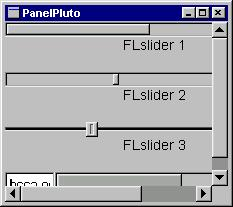
\includegraphics[scale=1]{flscroll} 


 FLscroll.
\subsection*{Examples}


  Here is an example of the flscroll opcode. It uses the files \emph{flscroll.orc}
 and \emph{flscroll.sco}
. 


 \textbf{Example 1. Example of the flscroll opcode.}

\begin{lstlisting}
/* flscroll.orc */
; Demonstration of the flscroll opcode which enables
; the use of widget sizes and placings beyond the
; dimensions of the containing panel
sr = 44100
kr = 441
ksmps = 100
nchnls = 1

FLpanel "Text Box", 420, 200, 50, 50
    iwidth = 420
    iheight = 200
    ix = 0
    iy = 0
    FLscroll iwidth, iheight, ix, iy
    ih3 FLbox "DRAG THE SCROLL BAR TO THE RIGHT IN ORDER TO READ THE REST OF THIS TEXT!", 1, 10, 20, 870, 30, 10, 100
    FLscrollEnd 
; End of panel contents
FLpanelEnd
; Run the widget thread!
FLrun

instr 1
endin
/* flscroll.orc */
        
\end{lstlisting}
\begin{lstlisting}
/* flscroll.sco */
; 'Dummy' score event of 1 hour.
f 0 3600
e
/* flscroll.sco */
        
\end{lstlisting}
\subsection*{See Also}


 \emph{FLgroup}
, \emph{FLgroupEnd}
, \emph{FLpack}
, \emph{FLpackEnd}
, \emph{FLpanel}
, \emph{FLpanelEnd}
, \emph{FLscrollEnd}
, \emph{FLtabs}
, \emph{FLtabsEnd}

\subsection*{Credits}


 Author: Gabriel Maldonado


 New in version 4.22


 Example written by Iain McCurdy, edited by Kevin Conder.
%\hline 


\begin{comment}
\begin{tabular}{lcr}
Previous &Home &Next \\
FLsavesnap &Up &FLscrollEnd

\end{tabular}


\end{document}
\end{comment}
